\documentclass[12pt,reqno]{amsart}

\usepackage{amsthm,amsmath,amssymb}
\usepackage{mathtools}
\usepackage{xcolor}
\usepackage{graphicx,wrapfig}
\usepackage[T1]{fontenc}
\usepackage{courier}
\usepackage{hyperref}
\hypersetup{
    hidelinks=true
}
\usepackage{array}
\usepackage{multirow}
\usepackage{listings}
\lstset{basicstyle=\ttfamily\footnotesize, columns=fullflexible, language=C, morekeywords={omp,task,private,pragma,parallel,reduction,single,nowait,num_threads}, numbers=left}
\newcommand{\code}[1]{\texttt{#1}}
\newcommand\MyBox[2]{
  \fbox{\lower0.75cm
    \vbox to 1.7cm{\vfil
      \hbox to 1.7cm{\hfil\parbox{1.4cm}{#1\\#2}\hfil}
      \vfil}%
  }%
}
\graphicspath{{./}}

\begin{document}

\begin{center}
\large\textbf{Assignment 3 \\ COMP529 Fall 2019 - Parallel Programming} \\
\normalsize\textbf{Erhan Tezcan 0070881 \\ 27.05.2020} \\
\end{center}


%\begin{figure}[h]
%\centering
%\begin{lstlisting}
%if (col < width && row < height) {
%  k = row * width + col;
%  image_k = image[k];
%  sdata[ty][tx] = image_k;
%}
%__syncthreads();
%\end{lstlisting}
%\caption{Loading phase of shared memory implementation.}
%\label{fig:reduc_2}
%\end{figure}

\section{Objective}

We are asked to implement an Iterative Sparse Matrix-Vector Multiplication, abbreviated as iSpMV. We have 4 versions of code in total:
\begin{enumerate}
	\item Serial
	\item MPI Implementation
	\item MPI+OpenMP Implementation
	\item Load Balanced MPI Implementation
\end{enumerate}
Version 2 is a modification of version 1, and versions 3 and 4 are modifications of version 2.

In this assignment, the matrix is a square matrix, say with dimensions $N\times N$. It is multiplied by a vector called \code{rhs} (right-hand side) with dimensions $N\times1$ and the \code{result} is the resulting vector with dimensions $N\times1$. For each iteration, we do this calculation and then copy \code{result} to the \code{rhs} for the next iteration. We are given the serial code, and will modify it for the remaining 3 versions specified above.

\section{Design \& Implementation}

In this section we will look at our implementations for each version other than the given serial version.

\subsection{Version 1: MPI}
The main idea of using MPI is to distribute the rows of the matrix intro processes. Basically, we will have a ``row per worker'' as \code{rpw} $=\lfloor N/p\rfloor$ where $N$ is the number of rows and $p$ is the number of processors. $p-1$ processes will get \code{rpw} rows to process, and the last process with id $p-1$ will be the master and get the remaining rows. This is done to overcome the cases when $N$ is not a multiple of $p$. Be aware that in this report $N$ is always the dimension of the matrix, and $p$ is always the number of processors, but may not be so in the code excerpts.

\subsubsection{Distribution of row offsets, column indices and column values at workers}
The master process has the full array of row offsets, column indices and column values because it is the process that reads the matrix. The worker processes only require the amount that they are going to process. In figure \ref{fig:allocs} we show how this distribution happens.

\begin{figure}[h]
\centering
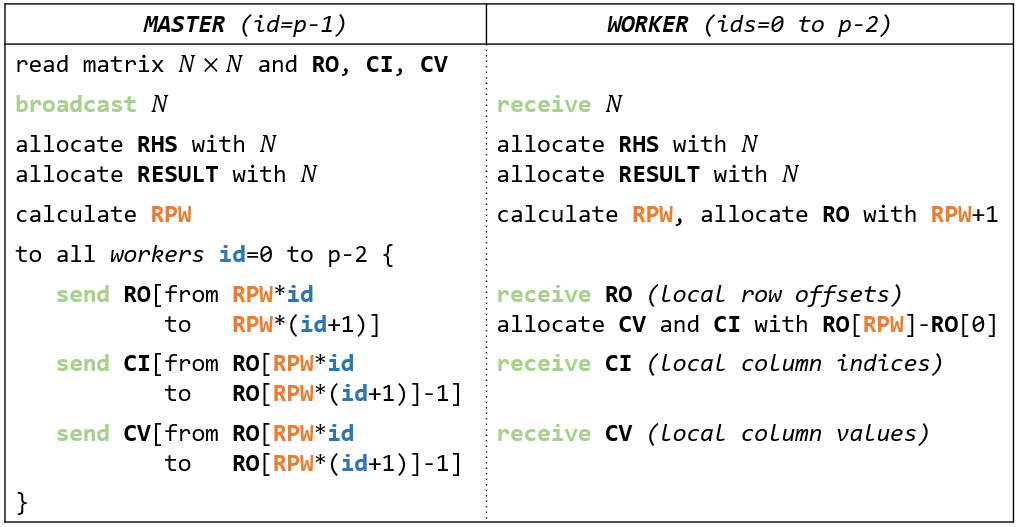
\includegraphics[width=\linewidth]{allocs.png}
\caption{Distribution of row offsets (RO), column indices (CI) and column values (CV) to workers.}
\label{fig:allocs}
\end{figure}

The workers do not know what $N$ is because they did not read the matrix, so first the master has to broadcast $N$. Then, the workers will allocate \code{rhs} and the \code{result} arrays with size $N$. They also know the number of processes so they can all calculate\code{rpw}. Note that in general, if master and worker can both calculate something, we prefer that over master doing the calculation and broadcasting it. This stems from the basic idea that computation costs less than communication. This is why for example \code{rpw} is calculated at all processes concurrently, rather than calculating it at master and then broadcasting it. After calculating \code{rpw}, the workers allocate \code{RO} with size \code{rpw+1} because they need one more row offset for the boundary. Workers then recieve the row offsets for their part as calculated by the \code{rpw}. The workers then allocate \code{CI} and \code{CV} with this information, more specifically by calculating \code{RO[rpw]-RO[0]}. Then they recieve those from the master.

The master sends these using \code{MPI\_Isend} but the workers recieve with \code{MPI\_Recv}. The reason workers are recieving with blocking functions is that they require these arrays to continue. However, the master should only wait for the completion of these sends after it has sent to all workers. If the master used \code{MPI\_Send} instead, all workers would recieve the messages one by one, which is not optimal at all.

\subsubsection{Calculations.}
We will show the calculations for both the master and the worker processes, though they are very similar.
\begin{figure}[h]
\centering
\begin{lstlisting}
myRow = rpw * taskid;
for (t = 0; t < time_steps; t++) {
  k = matrix.csrRowPtr[myRow];
  for(i = 0; i < matrix.m - myRow; i++) { 
    result[myRow + i] = 0.0;
    for (j = 0; j < matrix.csrRowPtr[myRow+i+1]-matrix.csrRowPtr[myRow+i]; j++) {
      result[myRow + i] += matrix.csrVal[k] * rhs[matrix.csrColIdx[k]];
      k++;
    }
  }
  MPI_Allgatherv(MPI_IN_PLACE, 0, MPI_DATATYPE_NULL,
                      result, recieveCounts, offsets, MPI_DOUBLE, MPI_COMM_WORLD);
  double* tmp = rhs; rhs = result; result = tmp; 
}
\end{lstlisting}
\caption{Calculations at master process.}
\label{fig:calc_master}
\end{figure}

\begin{figure}[h]
\centering
\begin{lstlisting}
myRow = rpw * taskid;
for (t = 0; t < time_steps; t++) {
  k = 0;
  for (i = 0; i < rpw; i++) {
    result[myRow + i] = 0.0;
    for (j = 0; j < csrRowPtr[i+1] - csrRowPtr[i]; j++) {
      result[myRow + i] += csrVal[k] * rhs[csrColIdx[k]];
      k++;
    }
  }
  MPI_Allgatherv(MPI_IN_PLACE, 0, MPI_DATATYPE_NULL, 
                       result, recieveCounts, offsets, MPI_DOUBLE, MPI_COMM_WORLD);
  double* tmp = rhs; rhs = result; result = tmp;
}	
\end{lstlisting}
\caption{Calculations at worker process.}
\label{fig:calc_worker}
\end{figure}
From figures \ref{fig:calc_master} and \ref{fig:calc_worker} the differences we see are all about the indexing. For example, \code{k} starts at 0 for the workers but it starts at \code{matrix.csrRowPtr[myRow]} for the master. This is because the workers do the calculations on their local arrays, which starts at $0$, but the master operates on the full array so it can't start at 0, it should start at it's own index which is given by \code{myRow}. Also notice how master thread works on \code{matrix.m - myRow} amount of rows, taking into account the remainder part of the rows in case the number of rows is not a multiple of the number of processors. 

\subsubsection{Usage of \code{MPI\_Allgatherv}.}
As we can see from figures  \ref{fig:calc_master} and \ref{fig:calc_worker}, we do the gathering with \code{MPI\_IN\_PLACE}. This is because we do not care about the part of the \code{result} that we do not operate on, and we are sure that other processes will not overwrite our results, so we can just gather to the array we already have, instead of creating another send buffer. The second and third parameters are ignored. Our recieving buffer is \code{result} array, as expected.

The \code{recieveCounts} and \code{offsets} are calculated by all processess concurrently, as shown in figure \ref{fig:calc_rcvoff}.
\begin{figure}[h]
\centering
\begin{lstlisting}
for (i = 0; i<numtasks - 1; i++) {
  recieveCounts[i] = rpw;
}
recieveCounts[numtasks - 1] = matrix.n - rpw * master;

offsets[0] = 0;
for (i = 1; i<numtasks; i++) {
  offsets[i] = offsets[i-1] + recieveCounts[i-1];
}
\end{lstlisting}
\caption{Calculations of \code{recieveCounts} and \code{offsets}.}
\label{fig:calc_rcvoff}
\end{figure}

Here, \code{master} is the id of the master process, which all processess know. Note that since \code{MPI\_Allgatherv} is a blocking function, we do not need any other synchronization here.

\subsubsection{Graceful termination}
Another important aspect of MPI programming is that, if there is an error that requires the program to abort, and this happens at the master process only, we should let all workers to know that the program is to abort, and everyone should call \code{MPI\_Finalize}. 
There is only one error that does not requires this, and that is because it is checked before \code{MPI\_Init}, it is the check for number of command line arguments. The other errors are only possible in the master process, and these are:
\begin{itemize}
	\item Error during reading the matrix file,
	\item If the read matrix is not a square matrix,
	\item If the number of processors are more than number of rows.
\end{itemize}
To do a graceful termination in presence of one of these errors, all processes store a variable called \code{proceedCode}, initialized to \code{DO\_PROCEED} which is just a macro. If there is an error, the master process sets this variable to \code{DO\_NOT\_PROCEED} and then broadcasts it to all workers, then calls \code{MPI\_Finalize} and returns with \code{EXIT\_FAILURE}. If there was no error, the master still broadcasts this variable with the value \code{DO\_PROCEED}. The worker processes expect this broadcast, and if they receive \code{DO\_PROCEED} they will continue, but if they receive \code{DO\_NOT\_PROCEED} they will call \code{MPI\_Finalize} and then return with \code{EXIT\_FAILURE}.

\subsubsection{Minor Improvements}
\label{sec:minor}
In the serial code, copying from \code{result} to \code{rhs} is done by iterating over the array and copying the \code{result} to \code{rhs}. However, we never actually read from the \code{result}, we only write to it in these calculations. Therefore, instead of copying, we could just do a pointer swap, which reduces the complexity of swapping from $O(n)$ to $O(1)$.

In loop declarations are removed and indexing variables such as \code{i, j, k, t} are moved to the top. This is known to increase performance as the number of iterations grow.

In the third part of every for loop (where we increment the index variable) we use pre-increment (\code{++i}) instead of post-increment (\code{i++}). This is probably not even noticable, but we still do it.

\subsection{Version 2: MPI + OpenMP}
In this version, we will do some improvements using OpenMP, over the existing MPI code we have and explained above. Note that we are aiming to use 16 processing units in total, so if we have 4 processors with MPI, this means we can create 4 threads each, because $4\times4=16$. In the code, this is done by the line \code{int numthreads = MAX\_NUM\_OF\_PROCESSORS / numtasks;} where \code{MAX\_NUM\_OF\_PROCESSORS} is 16. In all directives we have two clauses:
\begin{itemize}
	\item \code{num\_threads(numthreads)}
	\item \code{if(numthreads > 1)}
\end{itemize}
We use these clauses to ensure we use the correct amount of threads and do not waste performance for overhead when \code{numthreads} is 1. In the code, we can use thread-level parallelism for few loops other than the calculation phase, but for the sake of this report we will only talk about the calculations and how we parallelize them. Compared to the previous version, we will have a different type of indexing for the variable \code{k}. Notice that for the master process, \code{k} is initialized to \code{ matrix.csrRowPtr[myRow]} and for other workers it is intialized to 0. Then, as the loop progresses, we increment \code{k} one by one. Since the thread-level parallel version will process few rows at once, such sequential incremention will not work. Therefore we slightly changed the calculation part so that every \textbf{thread} initializes \code{k} to meet the index of the specified row.

\begin{figure}[h]
\centering
\begin{lstlisting}
myRow = rpw * taskid;
for (t = 0; t < time_steps; ++t) {	
  #pragma omp parallel for num_threads(numthreads) 
                               if(numthreads > 1) private(j, k)
  for (i = 0; i < matrix.m - myRow; ++i) { 
    k = matrix.csrRowPtr[myRow + i];
    result[myRow + i] = 0.0;
    for (j = 0; j < matrix.csrRowPtr[myRow+i+1]-matrix.csrRowPtr[myRow+i]; ++j) {
      result[myRow + i] += matrix.csrVal[k + j] * rhs[matrix.csrColIdx[k + j]];
    }
  }
  MPI_Allgatherv(MPI_IN_PLACE, 0, MPI_DATATYPE_NULL, 
                       result, recieveCounts, offsets, MPI_DOUBLE, MPI_COMM_WORLD);
  double* tmp = rhs; rhs = result; result = tmp;
}
\end{lstlisting}
\caption{Calculations at master process with OpenMP.}
\label{fig:calc_master_openmp}
\end{figure}

\begin{figure}[h]
\centering
\begin{lstlisting}
myRow = rpw * taskid;
for (t = 0; t < time_steps; ++t) {
  #pragma omp parallel for num_threads(numthreads)
                               if(numthreads > 1) private(j, k)
  for (i = 0; i < rpw; ++i) {
    k = csrRowPtr[i] - csrRowPtr[0];
    result[myRow + i] = 0.0;
    for (j = 0; j < csrRowPtr[i+1] - csrRowPtr[i]; ++j) {
      result[myRow + i] += csrVal[k + j] * rhs[csrColIdx[k + j]];
    }
  }
  MPI_Allgatherv(MPI_IN_PLACE, 0, MPI_DATATYPE_NULL, 
                       result, recieveCounts, offsets, MPI_DOUBLE, MPI_COMM_WORLD);
  double* tmp = rhs; rhs = result; result = tmp;
}	
\end{lstlisting}
\caption{Calculations at worker process with OpenMP.}
\label{fig:calc_worker_openmp}
\end{figure}

In figures \ref{fig:calc_master_openmp} and \ref{fig:calc_worker_openmp} we see the calculations. Most of it is similar to figures \ref{fig:calc_master} and \ref{fig:calc_worker}, except \code{k}. Notice how for the first row of every worker, \code{k} is 0 because the allocations are specific for every worker, but for the master \code{k} is initially \code{matrix.csrRowPtr[myRow]} because it is operating on the whole matrix data structure.

\section{Version 3: MPI with Load Balance}
In this version, we modify the code in version 1 such that the workers will get an approximately equal amount of work. This is done by distributing the work with respect to number of non-zeros rather than rows. The code is mostly same, the main difference is the rows per worker variable. In version 1, rows per worker, stored as \code{rpw}, was calculated by all workers as $=\lfloor N/p\rfloor$. This divided the rows only. Now, to balance the load on all workers, we will divide with respect to the number of non-zeros per worker. 

The master process holds the entirety of row offsets array, and using this array the master process will calculate the number of non-zeros and it's respective row counts, then distribute them to workers. In figure \ref{calc_nnz} we see how this happens. 
\begin{figure}[h]
\centering
\begin{lstlisting}
int nnz_tmp, rpw_tmp;
j = 0;
for (i = 0; i<numtasks-1; i++) {
  nnz_tmp = 0;
  rpw_tmp = 0;
  while (nnz_tmp < avgnnzpw && j < matrix.n) {
    nnz_tmp += matrix.csrRowPtr[j+1] - matrix.csrRowPtr[j];
    rpw_tmp++;	
    j++;
  }
  recieveCounts[i] = rpw_tmp;		
}
... // offsets are calculated as shown before
recieveCounts[numtasks-1] = matrix.n - offsets[numtasks-1];
\end{lstlisting}
\caption{Calculation of \code{recieveCounts} at master process.}
\label{fig:calc_nnz}
\end{figure}
Notice that we use the \code{recieveCounts} array for this part, and we use the same array for \code{MPI\_Allgatherv}. This is intuitive, since during the gathering each process get's as much as they are assigned rows. In the algorithm, we basically sum the number of non-zeros as we iterate over the rows, and when we exceed the average number of non-zeros per worker \code{avgnnzpw}, which is calculated as $=\lfloor NNZ/p\rfloor$, we assign the seen amount of rows to the current worker, and reset our variables for the next worker. We also ignore the master process during this loop, because we assign it's part later after we calculate the offsets, with the same algorithm we have given in figure \ref{fig:calc_rcvoff}. The last value in the \code{offsets} array gives us the starting row of the master process. We use this information to calculate how many rows are left for the master process.

The next thing we have to consider is that, in version 1, all workers found their starting row by simply calculating $\code{rpw * taskid}$ but we can't do that here because we do not assume all workers except the master have same amount of rows. The master needs to know the starting rows for all workers in particular for the distribution of \code{RO}, \code{CI} and \code{CV}. For this purpose, the master can just use the \code{offsets} array!

\section{Performance}

In this section we will discuss the performance, and show graphics regarding how each version compares to eachother.

\subsection{Validation \& Correctness}
Before we begin to compare our algorithms we first have to check for their correctness. For this purpose, we used our own small $4\times4$ matrix, taken directly from slide 35 of the Lecture Slide \#23 - Application Patterns. In our codes, we have a macro named \code{VERBOSE}, where if set to 1 makes the program print out contents such as \code{RO}, \code{CI}, \code{CV}, \code{recieveCounts} and \code{offsets} for each task if required. If we set \code{VERBOSE} to 2, we see the sum of first 100 or less values in the result array. We make this modification in the serial code too. We check the correctness of our algorithm by seeing the same sum result for all programs. In our submission, this macro is set to 0, which makes the compiler ignore all these extra print commands.

\subsection{Performance Analysis}
We will show both the calculation times and speedups for two matrices: \textit{Cube Coup dt6}\footnote{\url{https://sparse.tamu.edu/MM/Janna/Cube\_Coup\_dt6.tar.gz}} and \textit{Flan 1565}\footnote{\url{https://sparse.tamu.edu/MM/Janna/Flan\_1565.tar.gz}}.

\begin{figure}[h]
\centering
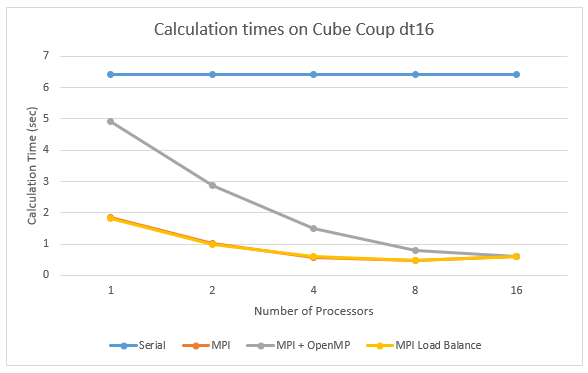
\includegraphics[width=\linewidth]{calc_coup.png}
\caption{Calculation times on \textit{Cube Coup dt6} matrix.}
\label{fig:calc_coup}
\end{figure}

\begin{figure}[h]
\centering
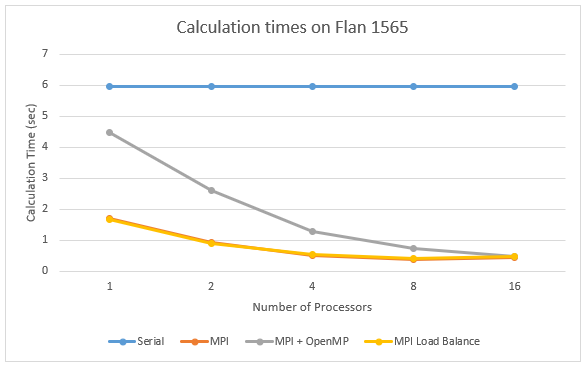
\includegraphics[width=\linewidth]{calc_flan.png}
\caption{Calculation times on \textit{Flan 1565} matrix.}
\label{fig:calc_flan}
\end{figure}

\begin{figure}[h]
\centering
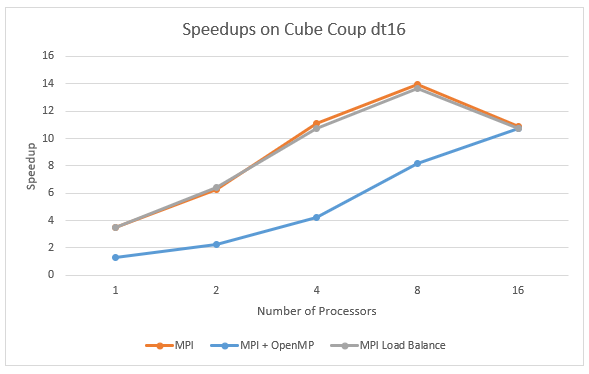
\includegraphics[width=\linewidth]{speedup_coup.png}
\caption{Speedups on \textit{Cube Coup dt6} matrix.}
\label{fig:speedup_coup}
\end{figure}

\begin{figure}[h]
\centering
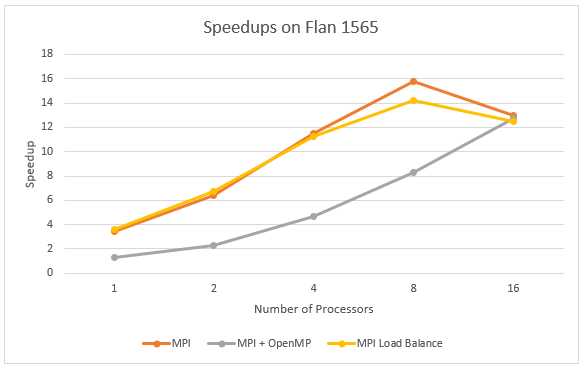
\includegraphics[width=\linewidth]{speedup_flan.png}
\caption{Speedups on \textit{Flan 1565} matrix.}
\label{fig:speedup_flan}
\end{figure}

In figures \ref{fig:calc_coup} and \ref{fig:calc_flan} we see how the calculation time varies for all versions and processor counts. In figures \ref{fig:speedup_coup} and \ref{fig:speedup_flan} we see how the speedup varies for all versions and processor counts, we did not include the serial code here since it would have a speedup of 1. We observe that all 3 parallel versions start with a better performance, and meet at approximately same performance level at 16 processors. We also see that MPI+OpenMP performs worse than the MPI at almost all variations of processor count. An explanation for this observation would be that when we use processes, we have them working on their own address space sequentially, but when we are working with threads within a processor, we might have an issue with cache locality. Since there is a lot of data to be processed and a relatively low number of threads, the effect of cache locality is amplified. MPI and MPI+OpenMP versions are expected to meet at 16 processors because the code is written in a way that OpenMP will not create a parallel region if the number of threads per processor is 1. We have explained this in MPI+OpenMP section. In other words, these two versions are identical at 16 processors. 

We also observe that MPI and MPI with Load Balance both perform almost equally. Their performance actually depends on the matrix at hand, and in this case we realize that when we divide the workload with respect to rows, or with respect to number of non-zeros, the distributed workload is more or less same. This means that the nonzeros in the matrix are almost equally distributed among the rows. Looking at the figures above, we can say that this holds for both matrices which we performed upon. We will explain why 16 processors perform worse than 8 processors in the next section. 

Regarding the fact that our parallel implementations with 1 process still perform better than serial: it could be because of the minor improvements we made, as discussed in section \ref{sec:minor}. These minor improvements apply to each iteration in every loop, which amplifies the performance gain for huge number of iterations. The most important one among them is the pointer swap instead of copying the array.

\subsection{Message Counts}
Let us see how many messages are passed around. We will ignore the \code{proceedCode} broadcast message because it is irrelevant to the application. For all versions, the first message is the broadcasting of matrix dimension $N$. In version 3, we also broadcast the \code{recieveCounts} array shortly after $N$. Then, in all versions, each process gets 3 messages, one for each of \code{RO}, \code{CI} and \code{CV} as seen in figure \ref{fig:allocs}. During the calculation phase, we only use \code{MPI\_Allgatherv} in each timestep. These are all the messages in our program.

The reason why 16 processes perform worse than 8 could be that during the gathering operation, the network bandwidth can't handle the transfer of that much data. Note that we allgather the \code{result}, whose size depends on the matrix. However, more processes mean that this array must be transferred to more processes, and this is probably why we observe the drop in performance. Note that MPI+OpenMP is an exception for 16 processes case, having performed better than it's 8 process version, however as we already said the 16 process version of MPI+OpenMP behaves identical to 16 processes MPI only.

\section{Acknowledgements}
I would like to include my thanks for this course in this part of the report, being that this is the last task regarding this course. I deeply thank to all teaching assistants Palwisha Akhtar and Muhammad Aditya Sasongko and our dear instructor Didem Unat. This course not only improved my parallel computation knowledge, but it increased my familiarity with compute clusters, command line interface and gave me the opportunity to take a deeper look in high performance computing area. \textit{Thank you!}

\end{document}